%
% Niniejszy plik stanowi przykład formatowania pracy magisterskiej na
% Wydziale MIM UW.  Szkielet użytych poleceń można wykorzystywać do
% woli, np. formatujac wlasna prace.
%
% Zawartosc merytoryczna stanowi oryginalnosiagniecie
% naukowosciowe Marcina Wolinskiego.  Wszelkie prawa zastrzeżone.
%
% Copyright (c) 2001 by Marcin Woliński <M.Wolinski@gust.org.pl>
% Poprawki spowodowane zmianami przepisów - Marcin Szczuka, 1.10.2004
% Poprawki spowodowane zmianami przepisow i ujednolicenie 
% - Seweryn Karłowicz, 05.05.2006
% Dodanie wielu autorów i tłumaczenia na angielski - Kuba Pochrybniak, 29.11.2016

% dodaj opcję [licencjacka] dla pracy licencjackiej
% dodaj opcję [en] dla wersji angielskiej (mogą być obie: [licencjacka,en])
\documentclass[licencjacka,en]{pracamgr}
\usepackage{hyperref}  % Enables clickable links
\usepackage{xcolor}    % Allows hyperlink color customization
\usepackage{graphicx}
\usepackage{listings}
\usepackage{minted}
\usepackage[toc,page]{appendix}
\usepackage{algorithm}
\usepackage{algpseudocode}
\usepackage{amsmath}


% Define JSON formatting style for listings
\lstdefinelanguage{json}{
    basicstyle=\ttfamily\small,
    numbers=left,
    numberstyle=\tiny,
    stepnumber=1,
    showstringspaces=false,
    breaklines=true,
    frame=single,
    backgroundcolor=\color{gray!10},
    keywordstyle=\color{blue},
    stringstyle=\color{red}
}

% Set hyperlink colors
\hypersetup{
    colorlinks=false,
    urlcolor=blue
}

% Dane magistranta:
\autori{Szymon Kozłowski}{448304}
\autorii{Gustaw Blachowski}{448194}
\autoriii{Kamil Dybek}{448224}
\autoriv{Natalia Junkiert}{448267}

\title{Using machine learning models for processing the data presented to the user by mobile devices.}

\tytulang{Using machine learning models for processing data presented to user by mobile devices.}
\titlepl{Wykorzystanie modeli uczenia maszynowego do przetwarzania danych zaprezentowanych użytkownikowi przez urządzenie mobilne.}

%kierunek: 
% - matematyka, informacyka, ...
% - Mathematics, Computer Science, ...
\kierunek{Computer Science}

% informatyka - nie okreslamy zakresu (opcja zakomentowana)
% matematyka - zakres moze pozostac nieokreslony,
% a jesli ma byc okreslony dla pracy mgr,
% to przyjmuje jedna z wartosci:
% {metod matematycznych w finansach}
% {metod matematycznych w ubezpieczeniach}
% {matematyki stosowanej}
% {nauczania matematyki}
% Dla pracy licencjackiej mamy natomiast
% mozliwosc wpisania takiej wartosci zakresu:
% {Jednoczesnych Studiow Ekonomiczno--Matematycznych}

% \zakres{Tu wpisac, jesli trzeba, jedna z opcji podanych wyzej}

% Praca wykonana pod kierunkiem:
% (podać tytuł/stopień imię i nazwisko opiekuna
% Instytut
% ew. Wydział ew. Uczelnia (jeżeli nie MIM UW))
\opiekun{Jacek Sroka PhD\\
  Institute of Informatics\\
  }

% miesiąc i~rok:
\date{\today}

%Podać dziedzinę wg klasyfikacji Socrates-Erasmus:
\dziedzina{ 
%11.0 Matematyka, Informatyka:\\ 
%11.1 Matematyka\\ 
%11.2 Statystyka\\ 
%11.3 Informatyka\\ 
11.4 Artificial Intelligence\\ 
%11.5 Nauki aktuarialne\\
%11.9 Inne nauki matematyczne i informatyczne
}

%Klasyfikacja tematyczna wedlug AMS (matematyka) lub ACM (informatyka)
\klasyfikacja{
  I.2.7: Natural Language Processing\\
  H.3.3: Information Search and Retrieval}

% Słowa kluczowe:
\keywords{LLM, NLP, BERT, Android, Edge-device, Fine-Tuning}

% Tu jest dobre miejsce na Twoje własne makra i~środowiska:
\newtheorem{defi}{Definicja}[section]

% koniec definicji
\let\cleardoublepage\clearpage
\begin{document}

\maketitle

%tu idzie streszczenie na strone poczatkowa
\begin{abstract}
In the era of rapidly evolving digital applications, traditional scraping techniques face increasing challenges in maintaining reliable data collection pipelines. Commissioned by Murmuras, a company specializing in commercial and scientific data analysis, in this project we present a novel approach to processing phone screen content, such as displayed social media posts and website advertisements. Our solution leverages Large Language Models (LLMs) running locally on the user's device to handle diverse data formats while ensuring that sensitive information remains protected. The primary application explored in this study is the extraction of discount coupons, demonstrating the feasibility of our method in identifying and structuring valuable content from varying digital sources. Furthermore, the system is designed to be easily adaptable to other use cases, such as analyzing users' political views. Additionally we explore usage of non-LLM models for the defined task. The results highlight the potential of LLM-driven content analysis as an alternative to conventional scraping techniques.
\raggedright
\end{abstract}

\tableofcontents
\listoffigures
\listoftables
\listofalgorithms

\chapter{Introduction}

\section{Project background and motivation}
With the rapid advancement of information technology, the Internet has become one of the most crucial facets for many businesses to perform marketing activities \cite{design_of_coupons}. One of the key marketing tools in business-to-consumer (B2C) e-commerce is the digital coupon \cite{targeted_reminders}. Compared to paper coupons, digital coupons are characterized by their wide reach, rapid distribution, and low spread costs. Furthermore, a key advantage of digital coupons is their ability to facilitate targeted marketing by offering personalized discounts to different customers, thereby increasing sales \cite{design_of_coupons}. 

Recent statistics underscore the significance of mobile devices in the domain of coupon distribution. For example, studies have shown that over 90\% of digital coupon users access their vouchers via smartphones \cite{emarketer_coupon_stats}, and similar figures are reported by other industry sources \cite{coupon_stats_2}. This high rate of mobile usage creates a pressing need for coupon analysis tools that are optimized for mobile platforms, ensuring that consumers receive timely and personalized offers regardless of their location or device.

Large Language Models (LLMs) have become a fundamental technique in contemporary machine learning, replacing previously utilized recurrent neural network (RNN) architectures in the field of natural language processing (NLP) \cite{li2024}. Subsequent research has demonstrated their applicability to structured input data \cite{sui2024}, such as screen views and coupons. Additionally, there have been efforts to integrate these models into web scraping pipelines \cite{scapegraph_repo}. 

In light of these trends, the company Murmuras has tasked us with developing a solution based on a machine learning model that can be deployed as a mobile application. This model will process input representing the user's onscreen view and extract digital coupons along with their relevant data. This solution must be capable of running locally on the device, ensuring efficient processing without relying on external servers. By leveraging advanced machine learning techniques, the app will handle the diverse formats and layouts of digital coupons, thus facilitating the collection of data regarding coupons.

\section{The definition of a coupon} 
A coupon is a physical piece of paper or digital voucher that can be redeemed for a financial discount when purchasing a product \cite{coupon_definition}. A coupon is characterized by a name, expiration date, and a discount type, e.g. '20\% off', 'buy 1 get 1 free', etc., however, not every coupon contains each of these features. Furthermore, coupons may contain numerous other features such as images and eligibility requirements. Henceforth, the term 'coupon' will refer exclusively to a digital coupon. The term 'conventional coupon' will refer to the traditional physical coupon. Examples of digital coupons encountered in mobile applications are presented in \ref{fig:example_coupons}

\begin{figure}[h]
    \centering
    \begin{minipage}{0.45\textwidth}
        \centering
        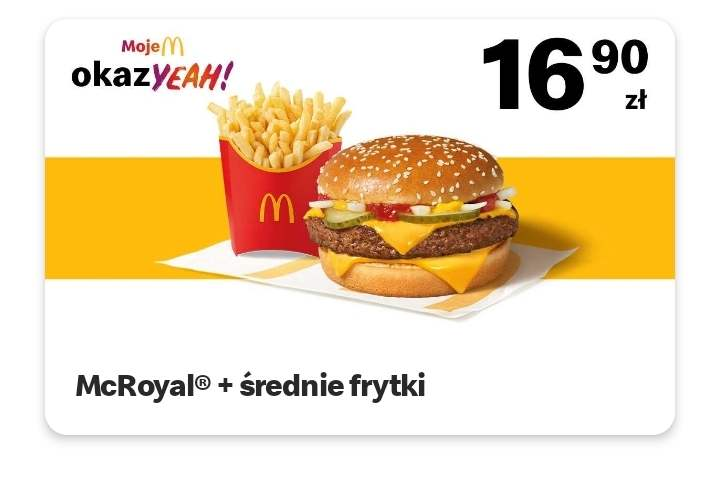
\includegraphics[width=\linewidth]{coupon1.jpg}
        \caption{Example coupon from fast-food restaurants chain mobile application}
    \end{minipage}
    \hfill
    \begin{minipage}{0.45\textwidth}
        \centering
        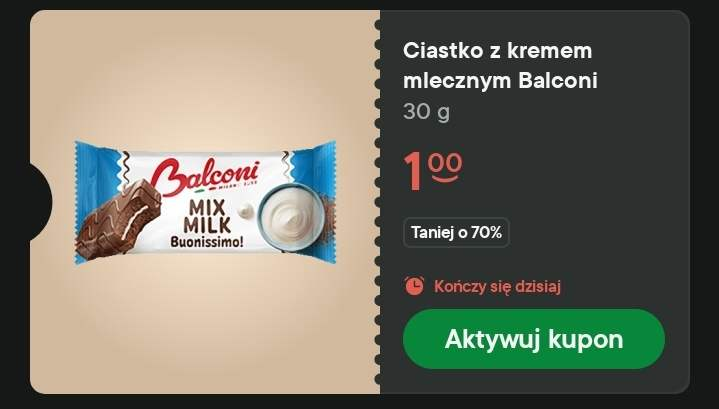
\includegraphics[width=\linewidth]{coupon2.jpg}
        \caption{Example coupon from grocery store mobile application}
    \end{minipage}
    \caption{Example digital coupons}
    \label{fig:example_coupons}
\end{figure}


\subsection{Our data model of digital coupon}
\label{sec:coupon_model}
In the following research we model a digital coupon as a collection of named fields:
\begin{enumerate}
    \item \textit{product\_name}: the name of the product,
    \item \textit{valid\_until}: the text representing the date of coupon expiration,
    \item \textit{discount\_text}: the text representing the discount offered to the user,
    \item \textit{activated}: either true or false, indicates whether the coupon has been activated,
\end{enumerate}
We allow for special \textit{null} value in the above fields in case no data is available. 

An example of a digital coupon represented in JSON format is shown in listing \ref{lst:coupon_example}:

\begin{lstlisting}[language=json, caption={Example of a digital coupon in JSON format}, label={lst:coupon_example}]
{
    "product_name": "Shampoo X",
    "valid_unitl": "2025-06-30",
    "discount_text": "20% OFF",
    "activated": true
}
\end{lstlisting}

\section{The Significance of the Digital Coupon}
The digital coupon is one of the most important tool in contemporary marketing strategies \cite{targeted_reminders}, therefore analyzing their lifecycle is essential to maximize their benefits. To facilitate such analyses, researchers collect various statistical metrics, including the fraction of redeemed coupons among all distributed coupons referred henceforth as redemption rate \cite{danaher2015} and customer engagement \cite{jayadharshini2023}, while also assessing their impact on sales performance \cite{jayadharshini2023}.  Additionally, studying competitors' digital coupon strategies enables businesses to identify market trends, adjust their promotional tactics, and maintain a competitive edge in the evolving digital marketplace. 

\subsubsection{Redemption Rate}  
The measurement of coupon redemption rates is primarily based on either survey data \cite{nayal2021} or controlled experimental studies \cite{danaher2015}. However, the company Murmuras \cite{murmuras} has introduced an alternative approach that enables the direct collection of coupon-related data from users' devices. This method utilizes a screen content scraping tool installed on the devices. Additionally, the tool has the ability to record user's actions.  Having access to all the user's interactions and visual changes in the layout, it is possible to detect the coupon redemption. This allows for large-scale data acquisition while reducing the costs associated with traditional survey-based methods.

\subsubsection{Customer Engagement and Impact on Sales}  

Customer engagement metrics, such as conversion rates and the effect of e-coupon issuance on sales, can potentially be measured using statistical analysis tools operating on the seller's website~\cite{seo2023}. The conversion rate is typically derived by tracking visitor activity, while the impact on sales is estimated by correlating the updated conversion rate with the frequency of coupon issuance.  

Although this approach provides valuable insights, it relies on direct collaboration with the coupon issuer and is constrained to a single webpage. Consequently, it is not applicable to our study, as we aim to analyze arbitrary mobile applications with diverse coupon designs.

\section{Problem Statement}

The objective of this work is to extract coupons visible to the user from the content displayed on a mobile device screen. The extracted coupons should be represented as a JSON list, with each entry conforming to the format specified in Section~\ref{sec:coupon_model}.  

The screen content is provided in the form of a \texttt{.CSV} file, which encodes an XML tree structure representing the underlying screen layout. Each row in this file corresponds to a single view element within the screen hierarchy~\cite{android_view}. The dataset includes at least the following attributes:  

\begin{enumerate}
    \item \textbf{view\_depth}: The depth of the view within the XML tree hierarchy.
    \item \textbf{text}: The textual content displayed to the user within the view.
    \item \textbf{id}: A unique identifier for a screen sample. Each sample consists of a set of views observed either simultaneously or in directly consecutive snapshots.
    \item \textbf{time}: The timestamp indicating when the view was recorded.
    \item \textbf{view\_id}: The unique identifier assigned to the view by the Android API.
\end{enumerate}

An example of the dataset to illustrate described format is provided in Table~\ref{tab:dataset_example}.

\begin{table}[h]
    \centering
    \begin{tabular}{|c|c|c|c|c|}
        \hline
        \textbf{view\_depth} & \textbf{text} & \textbf{id} & \textbf{time} & \textbf{view\_id} \\
        \hline
        2 & "50\% OFF" & 101 & 12:30:15 & \texttt{com.example.app:id/discount\_label} \\
        3 & "Buy 1 Get 1 Free" & 101 & 12:30:15 & \texttt{com.example.app:id/promo\_banner} \\
        2 & "Limited Offer" & 102 & 12:31:05 & \texttt{com.example.app:id/offer\_text} \\
        \hline
    \end{tabular}
    \caption{Example of dataset format representing screen content.}
    \label{tab:dataset_example}
\end{table}

Additional requirement is that the screen content processing will be performed exclusively on the end device to mitigate potential privacy concerns.

\section{Project goals}
The system will leverage machine learning to identify and structure relevant information while ensuring compatibility with mobile devices for enhanced accessibility and data privacy. The key goals of the project are as follows:

\begin{enumerate}
    \item A tool to process the data extracted from the device into a format suitable for use by the model.
    \item A machine learning tool for extracting the data that is of interest to us, such as the coupon name, expiration dates, prices, etc. The model should be capable of handling various coupon formats and layouts with high accuracy.
    \item An optional tool for post-processing the output data from the tool mentioned in the previous point into a common format.
    \item An application that runs the above three tools on a mobile device. (Optional)
    \item A key requirement is that the machine learning model must be deployable on the mobile device itself to guarantee data privacy.
\end{enumerate} 

\section{Potential applications of the project}
\subsection{Assessing coupon effectiveness}
The access to the content of mobile device screen allows us to list all the coupons seen by the user. Additionally, as we will retrieve information about coupon activation status, there will be possibility to track coupon redemptions by comparing the coupons models \textit{active} field.

Given that, our solution will aid businesses in analyzing consumer behavior and optimizing their marketing strategies. By facilitating the collection of data on coupon characteristics and their redemption rates, businesses will be able to assess the effectiveness of their coupon campaigns—determining whether they achieve the desired results. Additionally, large-scale analysis of coupon data can reveal valuable insights into purchasing patterns, preferred discount types, and the most appealing products or services.

\subsection{Market analysis and competitor monitoring}
Machine learning is proven to be a useful tool in the field of market competitors analysis but it requires significant amounts of data\cite{competitor_tariffs}.
The aforementioned gathering of data about displayed coupons can also be utilized in further monitoring of competitors' coupon strategies, their effectiveness, and whether they provide better discounts. Using machine learning to identify and analyze competitors' strategies is more cost-effective compared to exhaustive web scraping or mystery shopping \cite{competitor_tariffs}. This will enable businesses to make better informed decisions about their own marketing campaigns and provide a comprehensive understanding of the competitive landscape.

\chapter{BERT 2-stage architecture overview}
First introduced by Google in 2018~\cite{BERT_intro}, BERT models quickly became a standard in solving NLP-related tasks (as of 2025-04-04, it is the fourth most downloaded model on the HuggingFace~\cite{BERT_hf}). Its relatively small size (base model has around 110 mln parameters~\cite{BERT_hf}) as well as an easy to work with output format in case of the token classification fine-tuned versions were the reasons why BERT was our first pick for solving our problem. However, its advantages quickly started to be its disadvantages - input data proved to be too complex for the model to predict coupon attributes only inside them. This is why we propose a 2-stage architecture, similar to the region proposal~\cite{Region_proposal} architectures in computer vision, where regions would represent coupons, and the second stage would extract attributes from them. Thanks to it, we are able to minimize the number of false positives outside of coupons bodies.

\section{BERT family of models}
BERT model's popularity~\cite{BERT_hf} and age resulted in births of many variations of this architecture. Apart from obvious BERT-Large model (with over 300 mln parameters) and versions adopted for multilingual cases, attempts to update the architecture and to compress models were made. Former approaches beared fruit in RoBERTa models~\cite{RoBERTa}; BERT models which were extensively pretrained to match and even outperform base BERT.On the other hand, ALBERT~\cite{ALBERT} models were created to minimize the memory usage of the model, as well as the number of parameters (aroud 12 mln~\cite{ALBERT_hf}), while DISTILBERT~\cite{DISTILBERT} BLA BLA BLA SOMETHING TO DO. After reviewing available data, we decided to go with BERT base model. We decided that ALBERT model drop in performance is too big~\cite{BERT_comp}, while RoBERTa models weren't available for multiple languages~\cite{FBAIHF}. As a result, we ended up with the 179 mln parameter multilingual BERT model~\cite{BERT_multiling}.

\section{ModernBERT}
During our research phase, a new series of models was released: ModernBERTs~\cite{ModernBERTPaper}. While not being that much bigger than its predecessor (base model has 150 mln parameters~\cite{ModernBERThf}), it provides many improvements, like much bigger context (8192 tokens) and much faster processing. Additionally, it outperforms the base BERT model in many tasks. Hovewer, the lack of multilingual veriosn of the model, we ultimately decided to focus on its predecessor.

\section{2-stage architecture}
\begin{figure}
    \centering
    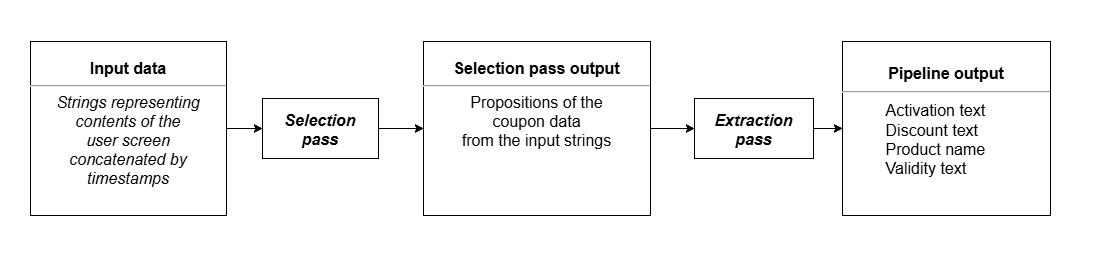
\includegraphics[width=1.0\linewidth]{zpp.png}
    \caption{Pipeline graph}
    \label{fig:zpp}
\end{figure}
Figure \ref{fig:zpp} represents the general structure of the system. It consists of:
\begin{enumerate}
    \item Input data: every frame registered on the user's phone is stored as an XML tree. This tree is later flattened into the CSV file, where entries belonging to the same frame have the same timestamp value. We use this value to gather and concatenate all text data present on the screen and feed it into the model.
    \item Selection pass: this is the first BERT multilingual model.
    \item Selection pass output: Selection pass produces data labeled by either B-COUPON, I-COUPON or UNKNOWN labels. B- and I-COUPON labels represent tokens contained in suspected coupons. These tokens are being concatenated back into strings, and then fed into the second BERT model.
    \item Extraction pass: this is the second BERT multilingual model.
    \item Pipeline output: extraction pass model outputs tokens labeled according to the field they belong in: Activation, discount, product or validity text. These tokens are being concatenated into strings based on those labels, and packed into jsons. As a result, we get the output format visible on the Listing \ref{list:pip-out}.
    \begin{center}
       \begin{listing}
            \begin{minted}[frame=single,
                           framesep=3mm,
                           linenos=true,
                           xleftmargin=21pt,
                           tabsize=4]{js}
            [
                {     
                    "ACTIVATION-TEXT" : string,
                    "DISCOUNT-TEXT" : string,
                    "PRODUCT-NAME" : string,
                    "VALIDITY-TEXT" : string,
                }
            ],
            ...
            \end{minted}
            \caption{Pipeline output} 
            \label{list:pip-out}
        \end{listing}
    \end{center}    
\end{enumerate}

\section{Training}
We decided to train both BERT models independently. This way, models are being penalized only for their mistakes. Otherwise, selection model loss function could be skewed by inacurate predictions of the extraction pass. On the other hand, extraction pass could learn on a skewed data, produced by learning selection pass. Additionally, separate fine-tunings were easier to both implement, and control.
\subsection{Experiments}
Both selection and extraction models were trained on a dataset consisting of data from 4 apps: DM, Lidl, Rewe and Rossman. Train-test split was 80-20, and evaluation was performed on every epoch. Following fine-tuning were performed for both models, with an assumtion that later, their performance will be measured with benchmark on the data from Edeka and Penny apps (to keep train and benchmark dataset sseparate):
\begin{enumerate}
\item General finetuning: the goal of this experiment was to check a general performance of models.
\item Per-app fine-tuning: the goal of this experiment was to see how will models fine-tuned on only one map behave on data from other apps (similaroty between datasets).
\item Incremental separate fine-tuning: the goal of this experiment was to check whether extending the knowledge of the model easily is possible. In order to check this, 4 models were produced for both passes: model fine-tuned only on DM app, model that was then further fine-tuned on Lidl app, then on Rewe and finally on Rossman.
\item Incremental combined fine-tuning: idea behind this experiment was similar to the incremental separate fine-tuning, hovewer here datasets were being concatenated, so that the first model would be fine-tuned only on DM, then it would be further fine-tuned on data from BOTH DM and Lidl and so on.
\end{enumerate}

\subsection{Selection pass specifics}
With selection pass, we decided to test two thing on top of a "normal" fine-tuning. First, we wanted to check if preserving the information about the xml tree in which the data was stored will help in finding coupons. For that, we prepared datasets in which strings representing screen content were wrapped in a json structure simulating said tree. Second, we wanted to check if balancing tokens distribution would help with the training. Main reason for this was the fact that early datasets that we received from the company had large amounts of data not belonging to any coupon. Additionally, json approach would introduce additional tokens, representing e.g. parenthesis that could also make it more difficult for the model to learn. However, mainly because later batches of data were free of these issues, this algorithm performance was ultimately non-satisfactory, and so it was abandoned. More on the topic can be found in Appendix \ref{AppA}.

\section{Fine-tuning results}
Czy/Co tu chcemy?

\section{Benchmark Results}
Czy/Co tu chcemy?

\begin{appendices}
\chapter{BERT Curriculum learning} \label{AppA}
In order to fight with the class imbalance in data provided by the Murmuras, as well as in the json approach for the selection BERT pass, we implemented a new algorithm, following ideas present in Curriculum Learning\cite{CurrLearn}. Idea behind this approach is to simulate the way humans learn: when we are young we are presented with easy problems, which complexity raises with time. In our case, this means that  at the beginning model would learn on data that has balanced classes of coupons and non-coupons, and with time, new dataset would be constructed that would contain more and more non-coupon labels. \\
Hovewer, while showing some promising behaviours, this approach was outclassed by default algorithms. Its main advantage was smoth and gradually descending evaluation loss, which would suggest that its not overfitting to the train data (which couldn't be said about the basic algorithm). Still, after 30 epochs, its accuracy and recall metrics were noticealby below the basic algorith, and so we decided to exclude it from further experiments.
\begin{figure}
    \centering
    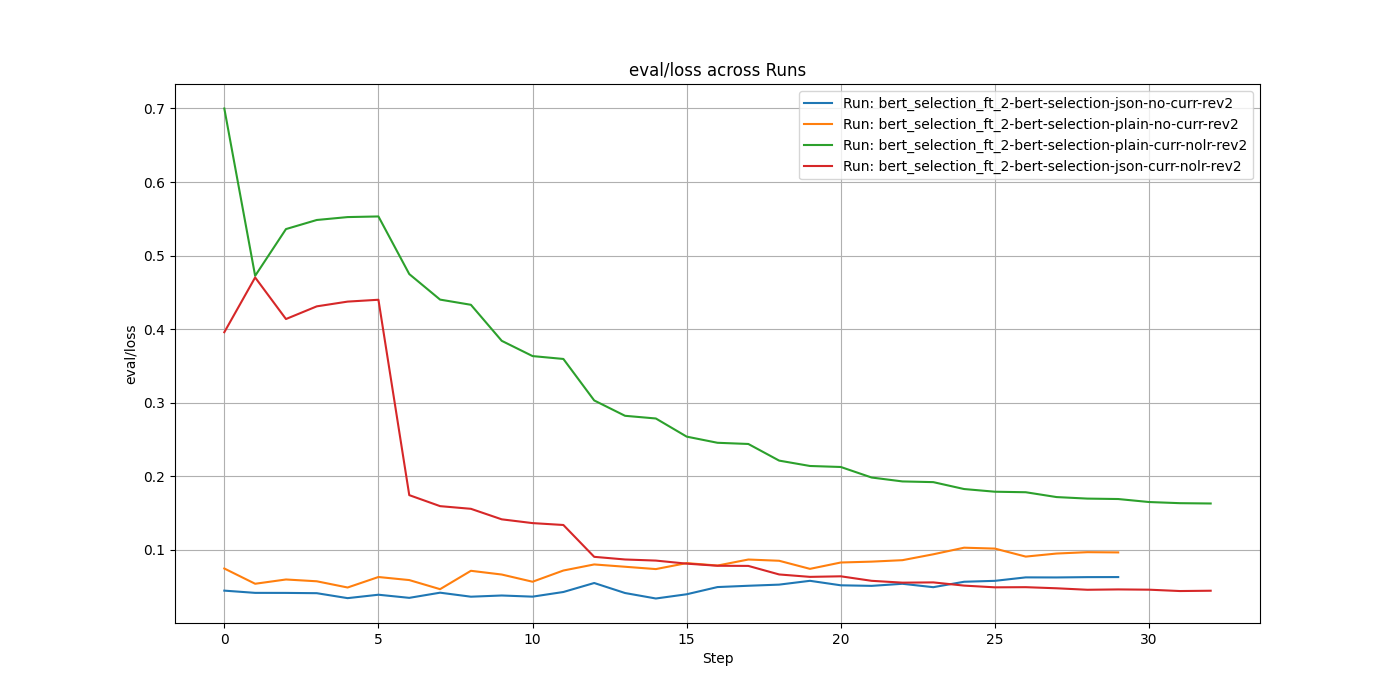
\includegraphics[width=1.0\linewidth]{evallossbert.png}
    \caption{Eval/loss statistics of selection pass algorithms during training}
    \label{fig:elb}
\end{figure}
\begin{figure}
    \centering
    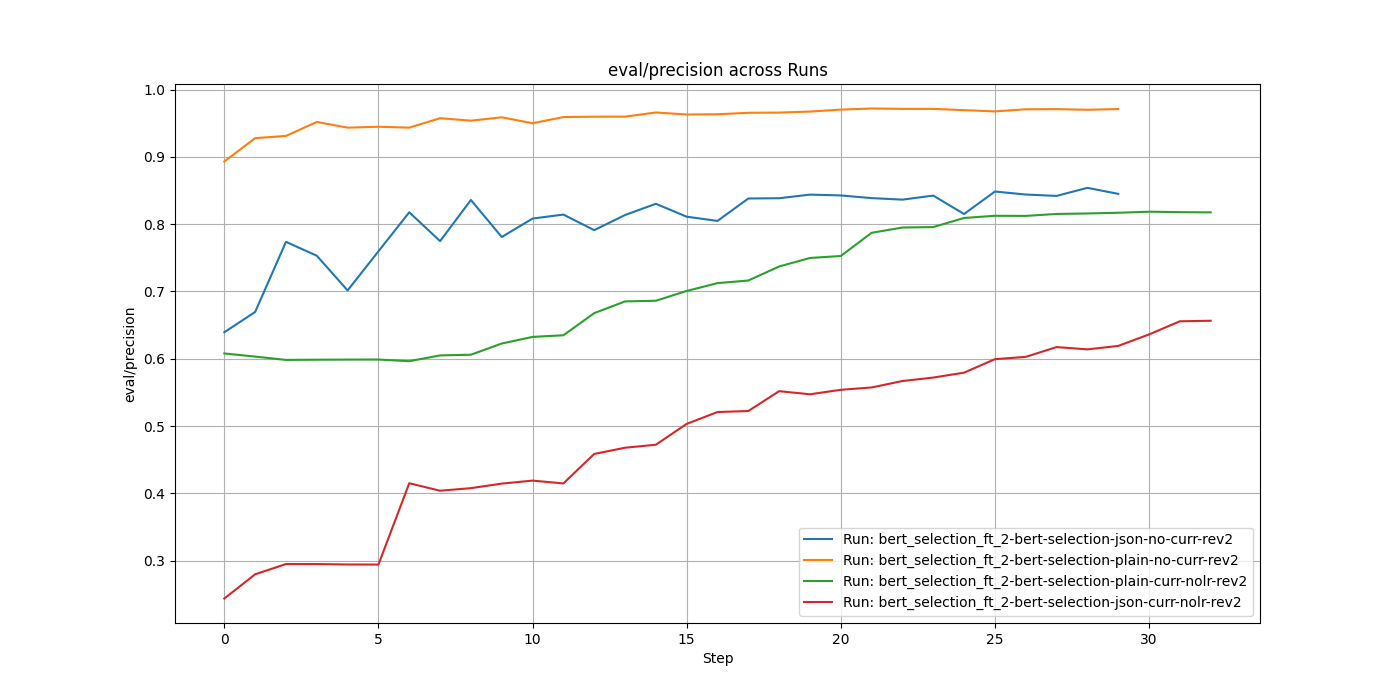
\includegraphics[width=1.0\linewidth]{evalprecbert.png}
    \caption{Eval/precision statistics of selection pass algorithms during training}
    \label{fig:epb}
\end{figure}
\begin{figure}
    \centering
    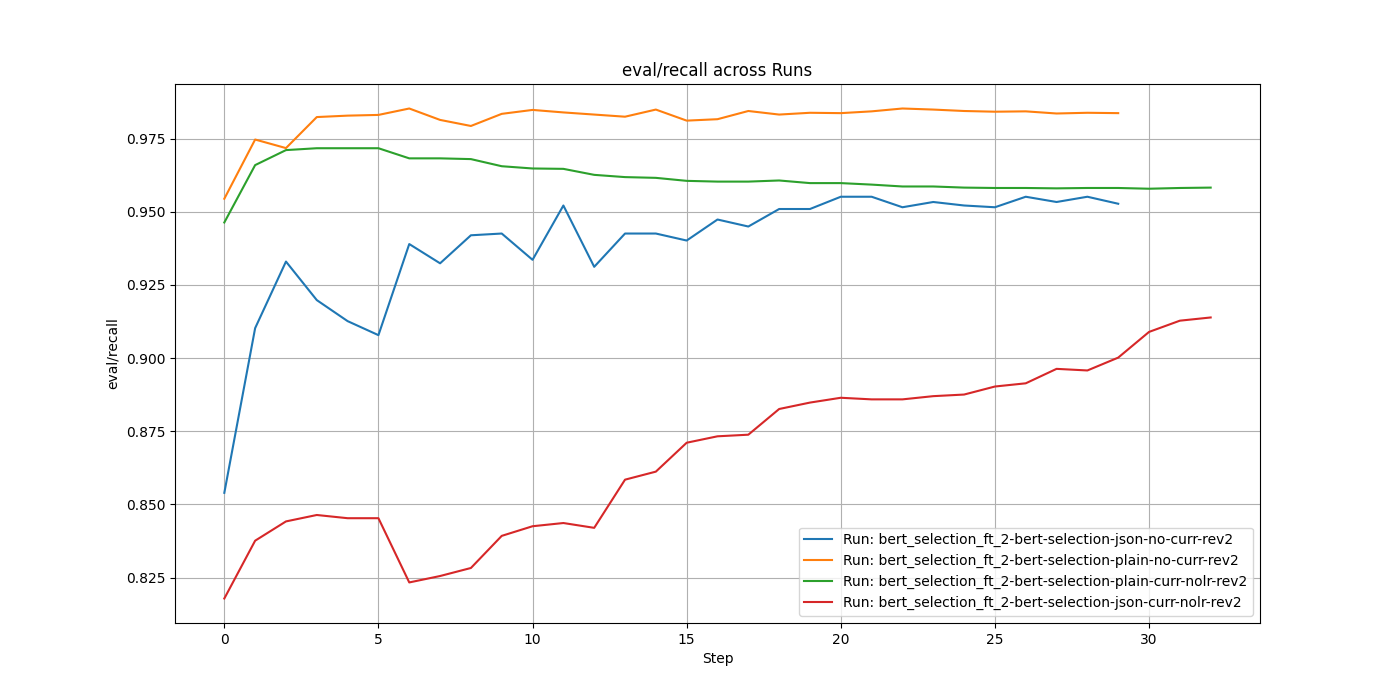
\includegraphics[width=1.0\linewidth]{evalrecbert.png}
    \caption{Eval/recall statistics of selection pass algorithms during training}
    \label{fig:erb}
\end{figure}



\begin{algorithm}
\caption{Curriculum Data Preparation Algorithm}
\begin{algorithmic}[1]
\Require Dataset $D$ with fields \texttt{texts}, \texttt{labels}
\Require Number of splits $S > 0$
\Ensure Sequence of training datasets

\State Initialize $\mathcal{R}_c \gets \{\}$, $\mathcal{R}_{\neg c} \gets \{\}$
\For{each row $r$ in $D$}
    \If{$r$ contains coupon labels}
        \State Extract spans of contiguous coupon tokens
        \State Add span info to $\mathcal{R}_c$
    \Else
        \State Add $r$ to $\mathcal{R}_{\neg c}$
    \EndIf
\EndFor

\State Store $\text{init\_len} \gets |\mathcal{R}_c|$
\For{each row $r$ in $\mathcal{R}_c$}
    \State Extend spans of $r$ proportionally using \textsc{ExtendSpans}
\EndFor
\State Yield initial dataset from $\mathcal{R}_c$

\For{$i = 1$ to $S-1$}
    \If{$i = S-1$}
        \State Append all of $\mathcal{R}_{\neg c}$ to $\mathcal{R}_c$
    \ElsIf{$i \bmod 2 = 0$}
        \State Append a subset of $\mathcal{R}_{\neg c}$ to $\mathcal{R}_c$
    \Else
        \For{each row $r$ in $\mathcal{R}_c$}
            \State Extend spans of $r$ proportionally
        \EndFor
    \EndIf
    \State Yield dataset from $\mathcal{R}_c$
\EndFor
\end{algorithmic}
\end{algorithm}

\begin{algorithm}
\caption{ExtendSpans Procedure}
\begin{algorithmic}[1]
\Procedure{ExtendSpans}{$spans, amount, max\_len$}
\If{$spans = \emptyset$}
    \State Create single span $[0, amount]$
\Else
    \State Distribute $amount$ evenly across spans
    \State Shift span boundaries without overlap
    \State Greedily expand remaining budget
\EndIf
\EndProcedure
\end{algorithmic}
\end{algorithm}

\end{appendices}

% \chapter{Technologies}
% \chapter{Architecture design}
% \chapter{Pipelines}
% \chapter{Benchmark}
% \chapter{Performance}
% \chapter{Possible extensions}
% \chapter{Conclusion}
% \chapter{Charts}

\begin{thebibliography}{99}

\addcontentsline{toc}{chapter}{Bibliography}
\raggedright

\bibitem{murmuras} 
\textit{Murmuras website}.  
\url{https://murmuras.com/}.  
[Accessed 2025-02-11].

\bibitem{seo2023}
\textit{Seo, D., \& Yoo, Y. (2023). Improving Shopping Mall Revenue by Real-Time Customized Digital Coupon Issuance. IEEE Access, 11, 7924–7932.}
\url{https://doi.org/10.1109/ACCESS.2023.3239425}

\bibitem{coupon_definition}
\textit{Britannica Dictionary definition of COUPON}.
\url{https://www.britannica.com/dictionary/coupon}.
[Accessed 2025-02-03].

\bibitem{nayal2021}
\textit{Nayal, P., \& Pandey, N. (2021). What Makes a Consumer Redeem Digital Coupons? Behavioral Insights from Grounded Theory Approach. *Journal of Promotion Management*, 28(3), 205–238.}
\url{https://doi.org/10.1080/10496491.2021.1989541}

\bibitem{danaher2015}
\textit{Danaher, P. J., Smith, M. S., Ranasinghe, K., \& Danaher, T. S. (2015). *Where, when, and how long: Factors that influence the redemption of mobile phone coupons.* *Journal of Marketing Research*, *52*(5), 710--725.}
\url{https://journals.sagepub.com/doi/full/10.1509/jmr.13.0341}

\bibitem{jayadharshini2023}
\textit{Jayadharshini, P., Sharon Roji, Priya. C, Lalitha, K., Santhiya, S., Keerthika, S., \& Abinaya, N. (2023). *Enhancing Retailer Auctions and Analyzing the Impact of Coupon Offers on Customer Engagement and Sales Through Machine Learning.* *2023 Intelligent Computing and Control for Engineering and Business Systems (ICCEBS)*, 1–6. }
\url{https://doi.org/10.1109/ICCEBS58601.2023.10448900}

\bibitem{design_of_coupons}
Xiong Keyi, Yang Wensheng
\textit{Research on the Design of E-coupons for Directional Marketing of Two Businesses in Competitive Environment}.
\url{https://www.sciencepublishinggroup.com/article/10.11648/j.ijefm.20200801.16}.
[Accessed 2025-02-04].

\bibitem{li2024}
\textit{Li, J. (2024). The evolution, applications, and future prospects of large language models: An in-depth overview. Applied and Computational Engineering 35, 234–244.}\url{https://doi.org/10.54254/2755-2721/35/20230399}

\bibitem{sui2024}
\textit{Sui, Y., Zhou, M., Zhou, M., Han, S., \& Zhang, D. (2024). Table meets LLM: Can large language models understand structured table data? A benchmark and empirical study. Proceedings of the 17th ACM International Conference on Web Search and Data Mining, 645--654.}

\bibitem{targeted_reminders}
Li Li, et. al.
\textit{Targeted reminders of electronic coupons: using predictive analytics to facilitate coupon marketing}.
\url{https://link.springer.com/article/10.1007/s10660-020-09405-4}.
[Accessed 2025-02-04].

\bibitem{competitor_tariffs}
Bernhard König, et. al.
\textit{Analysing competitor tariffs with machine learning}.
\url{https://www.milliman.com/en/insight/analysing-competitor-tariffs-with-machine-learning}.
[Accessed 2025-02-04].

\bibitem{ml_general}
Iqbal H. Sarker
\textit{Machine Learning: Algorithms, Real-World Applications and Research Directions}.
\url{https://link.springer.com/article/10.1007/s42979-021-00592-x}.
[Accessed 2025-02-05].

\bibitem{emarketer_coupon_stats}
Sara Lebow
\textit{How consumers access digital coupons}.
\url{https://www.emarketer.com/content/how-consumers-access-digital-coupons}.
[Accessed 2025-02-05].

\bibitem{coupon_stats_2}
\textit{Unveiling IT Coupons Trends and Statistics}
\url{https://www.go-globe.com/unveiling-it-coupons-trends-statistics/}.
[Accessed 2025-02-05].

\bibitem{android_view}
\textit{Android API Reference - View}
\url{https://developer.android.com/reference/android/view/View}
[Accessed 2025-03-11]

\bibitem{brinkmann2023}
\textit{Brinkmann, A., Shraga, R., Der, R. C., \& Bizer, C. (2023). Product Information Extraction using ChatGPT. arXiv preprint, arXiv:2306.14921.}
\url{https://arxiv.org/abs/2306.14921}

\bibitem{chatgpt_params}
\textit{Tom B. Brown, Benjamin Mann, Nick Ryder, Melanie Subbiah, Jared
Kaplan, Prafulla Dhariwal, Arvind Neelakantan, Pranav Shyam, Girish
Sastry, Amanda Askell, Sandhini Agarwal, Ariel Herbert-Voss, Gretchen
Krueger, Tom Henighan, Rewon Child, Aditya Ramesh, Daniel M.
Ziegler, Jeffrey Wu, Clemens Winter, Christopher Hesse, Mark Chen,
Eric Sigler, Mateusz Litwin, Scott Gray, Benjamin Chess, Jack Clark,
Christopher Berner, Sam McCandlish, Alec Radford, Ilya Sutskever, and
Dario Amodei. Language models are few-shot learners, 2020}

\bibitem{scapegraph_repo}
Marco Perini, Lorenzo Padoan, Marco Vinciguerra
\textit{Scrapegraph-ai}.
\url{https://github.com/VinciGit00/Scrapegraph-ai}.
[Accessed 2025-02-24].

\bibitem{ollama_repo}
\textit{Ollama}.
\url{https://github.com/ollama/ollama}.
[Accessed 2025-02-24].

\bibitem{scapegraph_usage}
Marco Perini, Lorenzo Padoan, Marco Vinciguerra
\textit{Scrapegraph-ai usage}.
\url{https://github.com/ScrapeGraphAI/Scrapegraph-ai?tab=readme-ov-file#-usage}.
[Accessed 2025-02-24].

\bibitem{scapegraph_sdks}
Marco Perini, Lorenzo Padoan, Marco Vinciguerra
\textit{Scrapegraph-ai API and SDKs}.
\url{https://github.com/ScrapeGraphAI/Scrapegraph-ai?tab=readme-ov-file#-scrapegraph-api--sdks}.
[Accessed 2025-02-24].

\bibitem{android_dev_site}
\textit{Android developer fundamentals website}.
\url{https://developer.android.com/guide/components/fundamentals}.
[Accessed 2025-02-24].

\bibitem{ios_dev_site}
\textit{Apple developer website}.
\url{https://developer.apple.com/develop/}.
[Accessed 2025-02-24].

\bibitem{omniparser_intro}
\textit{Yadong Lu, Jianwei Yang, Yelong Shen, and Ahmed Awadallah. Omni-
parser for pure vision based gui agent, 2024.}

\bibitem{cheng2024}
\textit{Cheng, K., Sun, Q., Chu, Y., Xu, F., Li, Y., Zhang, J., \& Wu, Z. (2024). SeeClick: Harnessing GUI Grounding for Advanced Visual GUI Agents. arXiv preprint, arXiv:2401.10935.} \url{https://arxiv.org/abs/2401.10935}

\bibitem{mobile_resources}
Xiang Li, et. al.
\textit{Large Language Models on Mobile Devices: Measurements, Analysis, and Insights}
\url{https://dl.acm.org/doi/10.1145/3662006.366205}

\bibitem{LinguaLinked}
Junchen Zhao, et. al.
\textit{LinguaLinked: A Distributed Large Language Model Inference System for Mobile Devices}
\url{https://arxiv.org/pdf/2312.00388}

\bibitem{sequence_matcher}
\textit{difflib — Helpers for computing deltas}
\url{https://docs.python.org/3/library/difflib.html}

\bibitem{francuz}
\textit{Deep Learning with Python}
\url{https://sourestdeeds.github.io/pdf/Deep%20Learning%20with%20Python.pdf}

\bibitem{nvidiaimage}
\textit{What’s the Difference Between Artificial Intelligence, Machine Learning and Deep Learning?}
\url{https://blogs.nvidia.com/blog/whats-difference-artificial-intelligence-machine-learning-deep-learning-ai/}

\bibitem{ibm_ai}
\textit{What is artificial intelligence (AI)?}
\url{https://www.ibm.com/think/topics/artificial-intelligence}

\bibitem{ibm_privacy}
\textit{Exploring privacy issues in the age of AI}
\url{https://www.ibm.com/think/insights/ai-privacy}

\bibitem{mycin}
\textit{MYCIN}
\url{https://www.britannica.com/technology/MYCIN}

\bibitem{supervised_ibm}
\textit{Supervised versus unsupervised learning: What's the difference?}
\url{https://www.ibm.com/think/topics/supervised-vs-unsupervised-learning}

\bibitem{benchmark} 
\textit{Computer Benchmark}.
\url{https://bhatabhishek-ylp.medium.com/benchmarking-in-computer-c6d364681512}.
[Accessed 2025-02-03].

\bibitem{not_sroka_vid} 
\textit{The privacy paradox with AI}.
\url{https://www.reuters.com/legal/legalindustry/privacy-paradox-with-ai-2023-10-31/}.
[Accessed 2025-03-24].

\bibitem{ai_scare2}
\textit{Beware the Privacy Violations in Artificial Intelligence Applications}
\url{https://www.isaca.org/resources/news-and-trends/isaca-now-blog/2021/beware-the-privacy-violations-in-artificial-intelligence-applications}
[Accessed 2025-04-01]

\bibitem{ai_scare3}
\textit{AI – the threats it poses to reputation, privacy and cyber security, and some practical solutions to combating those threats}
\url{https://www.taylorwessing.com/en/global-data-hub/2024/cyber-security---weathering-the-cyber-storms/ai---the-threats-it-poses-to-reputation}

\bibitem{ai_env_concerns}
\textit{AI has an environmental problem. Here’s what the world can do about that.}
\url{https://www.unep.org/news-and-stories/story/ai-has-environmental-problem-heres-what-world-can-do-about}
[Accessed 2025-03-24]

\bibitem{it_convergence} 
\textit{Top Use Cases of AI-Based Recommendation Systems}.
\url{https://www.itconvergence.com/blog/top-use-cases-of-ai-based-recommendation-systems/}.
[Accessed 2025-03-24].

\bibitem{builtin} 
\textit{ 14 Risks and Dangers of Artificial Intelligence (AI)}.
\url{https://builtin.com/artificial-intelligence/risks-of-artificial-intelligence}.
[Accessed 2025-03-24].

\bibitem{data_guard} 
\textit{The growing data privacy concerns with AI: What you need to know}.
\url{https://www.dataguard.com/blog/growing-data-privacy-concerns-ai/}.
[Accessed 2025-03-24].

\bibitem{transcend} 
\textit{Examining Privacy Risks in AI Systems}.
\url{https://transcend.io/blog/ai-and-privacy}.
[Accessed 2025-03-24].

\bibitem{ibm_vast_data} 
\textit{Exploring privacy issues in the age of AI}.
\url{https://www.ibm.com/think/insights/ai-privacy}.
[Accessed 2025-03-24].


\bibitem{forbes_dl_env}
\textit{Deep Learning’s Carbon Emissions Problem}.
\url{https://www.forbes.com/sites/robtoews/2020/06/17/deep-learnings-climate-change-problem/}.
[Accessed 2025-03-24].

\bibitem{nyt_el}
\textit{A.I. Could Soon Need as Much Electricity as an Entire Country}.
\url{https://www.nytimes.com/2023/10/10/climate/ai-could-soon-need-as-much-electricity-as-an-entire-country.html}.
[Accessed 2025-03-24].

\bibitem{sci_dir_comp}
\textit{Trends in AI inference energy consumption: Beyond the performance-vs-parameter laws of deep learning}.
\url{https://www.sciencedirect.com/science/article/pii/S2210537923000124#sec7}.
[Accessed 2025-03-24].

\bibitem{sci_am_co2}
\textit{A Computer Scientist Breaks Down Generative AI’s Hefty Carbon Footprint}.
\url{https://www.scientificamerican.com/article/a-computer-scientist-breaks-down-generative-ais-hefty-carbon-footprint/}.
[Accessed 2025-03-24].

\bibitem{water_scarcity}
\textit{AI Is Accelerating the Loss of Our Scarcest Natural Resource: Water}.
\url{https://www.forbes.com/sites/cindygordon/2024/02/25/ai-is-accelerating-the-loss-of-our-scarcest-natural-resource-water/}.
[Accessed 2025-03-24].

\bibitem{first}
\textit{AI has an environmental problem. Here’s what the world can do about that.}.
\url{https://www.unep.org/news-and-stories/story/ai-has-environmental-problem-heres-what-world-can-do-about}.
[Accessed 2025-03-24].

\bibitem{ibm_dl}
\textit{What is deep learning?}.
\url{https://www.ibm.com/think/topics/deep-learning}.
[Accessed 2025-03-24].

\bibitem{BERT_intro}
\textit{BERT: Pre-training of Deep Bidirectional Transformers for Language Understanding}.
\url{https://arxiv.org/abs/1810.04805v2}.
[Accessed 2025-04-04]

\bibitem{BERT_hf}
\textit{BERT model page on hf}.
\url{https://huggingface.co/google-bert/bert-base-uncased}.
[Accessed 2025-04-04]

\bibitem{Region_proposal}
\textit{Faster R-CNN: Towards Real-Time Object Detection with Region Proposal Networks}
\url{https://arxiv.org/abs/1506.01497}
[Accessed 2025-04-04]

\bibitem{RoBERTa}
\textit{RoBERTa: A Robustly Optimized BERT Pretraining Approach}.
\url{https://arxiv.org/abs/1907.11692}
[Accessed 2025-04-04]

\bibitem{ALBERT}
\textit{ALBERT: A Lite BERT for Self-supervised Learning of Language Representations}.
\url{https://arxiv.org/abs/1909.11942}
[Accessed 2025-04-04]

\bibitem{ALBERT_hf}
\textit{ALBERT model page on hf}.
\url{https://huggingface.co/albert/albert-base-v2}.
[Accessed 2025-04-04]

\bibitem{DISTILBERT}
\textit{DistilBERT, a distilled version of BERT: smaller, faster, cheaper and lighter}
\url{https://arxiv.org/abs/1910.01108}
[Accessed 2025-04-04]

\bibitem{BERT_comp}
\textit{Comparative Analysis of BERT Variants for Text Detection Tasks}
\url{https://www.researchgate.net/publication/385142549_Comparative_Analysis_of_BERT_Variants_for_Text_Detection_Tasks}
[Accessed 2025-04-04]

\bibitem{FBAIHF}
\textit{Facebook AI on HuggingFace}
\url{https://huggingface.co/FacebookAI}
[Accessed 2025-04-04]

\bibitem{BERT_multiling}
\textit{Multilingual BERT on HuggingFace}
\url{https://huggingface.co/google-bert/bert-base-multilingual-cased}
[Accessed 2025-04-04]

\bibitem{ModernBERTPaper}
\textit{Smarter, Better, Faster, Longer: A Modern Bidirectional Encoder for Fast, Memory Efficient, and Long Context Finetuning and Inference}
\url{https://arxiv.org/abs/2412.13663}
[Accessed 2025-04-05]

\bibitem{ModernBERThf}
\textit{ModernBERT on HiggingFace}
\url{https://huggingface.co/answerdotai/ModernBERT-base}
[Accessed 2025-04-05]

\bibitem{CurrLearn}
\textit{Curriculum learning}
\url{https://dl.acm.org/doi/abs/10.1145/1553374.1553380}
[Accessed 2025-04-07]


\end{thebibliography}

\end{document}


%%% Local Variables:
%%% mode: latex
%%% TeX-master: t
%%% coding: latin-2
%%% End: